\subsection{Simulation Results}
\label{sec:simulation}
%\Matt{BLUE: I would not mind removing this text. RED: I will likely remove this text}
%The simulation results are consistent across all the PARSEC benchmarks. The reason for this consistency is due to the similarity of the memory traces across the benchmarks. 

Given sufficient memory overhead, we see a consistent 25\% reduction in CPU cycles over the baseline simulation, with Coding Scheme I generally performing best. 

%\subsection{PARSEC Results}

The proposed memory system performs consistently across the PARSEC benchmarks, and the three proposed schemes yield similar results. Figure~\ref{fig:dedup_results} shows the simulation results for the dedup benchmark with a memory partition coefficient $r = 0.05$. The plot shows that the number of CPU cycles is reduced by $73\%--83\%$ once sufficient memory overhead $\alpha$ is used. 
%The lines on this figure and others show the number of CPU cycles needed for the Ramulator simulation to finish executing. 
We also see that the number of memory region switches performed by the dynamic encoder. When $\alpha = 1$, the number of switches is always zero as expected because the dynamic encoder never needs to switch regions. The performance remains consistent for $\alpha > 0.1$. With this amount of overhead, the memory system finds and encodes the two heavily accessed memory bands in each of the PARSEC benchmarks. This is because $\lfloor\frac{\alpha}{r}\rfloor = 2$, which means we can select $2$ regions to encode. 
%The number of coded region switches is evidence that at $\alpha = .05$ more memory is needed to see maximum benefits from the memory system. 
When $\alpha = 0.05$, the number of coded region switches is very high because the memory system vacillates between the two most heavily accessed bands. When $\alpha = .1$, both of them can be encoded. We see a small numbers of switches when $\alpha \geq 0.25$ because the memory system is encoding less heavily accesses memory bands with little impact on number of CPU cycles.


The heavily accessed memory bands are narrow, which suggests that decreasing the memory bank partition will result in similar performance improvements with a lower $\alpha$. Figure~\ref{fig:dedup_hundreth} shows that indeed $\alpha$ can be reduced by a factor of $5$ by also decreasing $r$ from $0.05$ to $0.01$.


%\subsection{PARSEC Augmentation}
%\subsection{Augmentation}

\subsubsection{Augmented PARSEC}

Results on the the augmented PARSEC traces show that our system improves over the baseline to a lesser extent.
%
%results significantly impact the Ramulator simulation results. Increasing the number of memory bands by splitting the dense bands results in an increased memory requirement to see improved performance. Introducing a ramp to the memory bands decreases the efficacy of the proposed memory system across all values of $\alpha$. \Ethan{highlight it's still good}
%
Figure~\ref{fig:vips_split_result} shows that for a large number of memory bands, we can achieve the same performance as before only by increasing the memory overhead or increasing the memory partition coefficient.
% The memory partition coefficient used here is $r = .05$, but as shown in Figures ~\ref{fig:dedup_results} and ~\ref{fig:dedup_hundreth} lowering the memory partition coefficient allows a lowering of $\alpha$ while achieving the same performance.

Figure~\ref{fig:vips_ramp_result} shows the results of the ramp augmentation. Here we see that our system struggles to adapt to a constantly changing primary access region. 

%The proposed memory system performace worse in this scenario. The number of memory region switches shows that the memory system struggles to handle the constantly changing location of the heavily accessed memory regions. 

In the other simulator results, we see that the number of memory region switches decreases as a function of $\alpha$. \Ethan{show this in the appendix or don't mention it at all.}

%The reason for this is that the memory system locates the heavily accessed memory regions and rarely switches away from them. Here, the memory system is constantly attempting to catch up with the heavily accessed memory region. {\color{blue}We note that the ramp covers a very large number of memory addresses, so the decrease in performance we observe would only effect programs which use very large portions of memory.} 

\begin{figure}[htbp]
		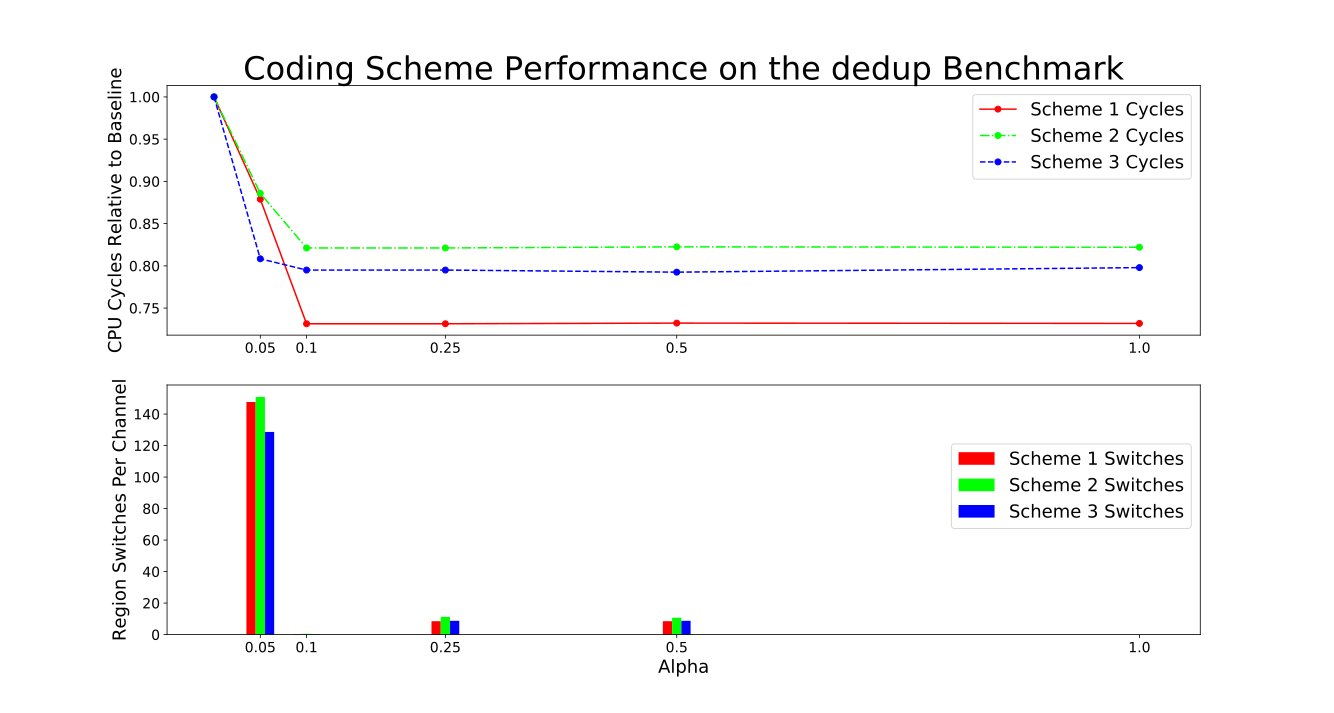
\includegraphics[width=\linewidth]{fig/dedup_benchmark_results.png}
		\caption{The simulation results for the dedup PARSEC benchmark. The line plot represents the number of CPU cycles needed and the bar plot represents the number of items the dynamic coding unit chooses to encode a new memory region. The results from the other PARSEC benchmarks are similar.}
		\label{fig:dedup_results}
\end{figure}

\begin{figure}[htbp]
		\includegraphics[width=\linewidth]{fig/dedup_hundreth.png}
		\caption{The simulation results for the same trace simulated in Figure~\ref{fig:dedup_results} but with a memory partition coefficient $r = .01$}
		\label{fig:dedup_hundreth}
\end{figure}

\begin{figure}[htbp]
		\includegraphics[width=\linewidth]{fig/vips_split_results.png}
		\caption{The simulation results of the augmented vips trace pictured in Figure~\ref{fig:vips_split}}
		\label{fig:vips_split_result}
\end{figure}

\begin{figure}[htbp]
		\includegraphics[width=\linewidth]{fig/vips_ramp_results.png}
		\caption{The simulation results of the augmented vips trace pictured in Figure~\ref{fig:vips_ramp}}
		\label{fig:vips_ramp_result}
\end{figure}


